\section{Infrastructure for Radioactive Source Calibration}\label{section:hf_exprimentalsetup}

\subsection{Source Driver System}
To perform calibration of the calorimeter with a radioactive source, a
specialized source driver system has been developed. It includes devices capable of inserting a long thin wire, approximately 11 m long, tipped with a point-like radioactive source into the HF source tubes embedded in the calorimeter. As the radioactive source moves through the HF absorber, gamma rays are emitted and consequently create Compton electrons, which in turn can generate Cherenkov photons inside the quartz fibers if they exceed the Cherenkov threshold. With the new HF PMTs, the quantum efficiency is such that 30\% of the photons reaching the PMT cathode face will actually be converted into the read out signal.

The thin wire, referred to as the source wire, used by the system is made of
stainless steel and has inner and outer diameters of 0.406 mm and 0.711 mm,
respectively. The end of the wire that penetrates the HF absorber, the front end,
is melted shut, shaped into a bullet nose, and chemically plated to reduce friction. The point-like radioactive source is inserted into the opposite end of
the wire, the back end, and held in place against the front end by a fine steel
piano wire. The outer source wire and inner piano wire are then crimped together at the back end in order to fix the position of the radioactive source.

A Lexan polycarbonate reel, belt driven by a DC reversible electric motor, is used
to insert or retract the source wire into or out of the calorimeter's source tubes.
The calorimeter's source tubes are coupled to acetal plastic tubing to mediate the
transfer of the source wire from the source driver into the absorber. The
transition between the plastic tube and the metal source tube typically involve
small-angle conical holes in brass that channel the source wire to the source tube.

The driver system also contains an additional electric motor that functions to
select the source tube into which to direct the source wire, an action referred
to as indexing. The position of the radioactive source, referred to as the reel position, is provided by an optical rotary
encoder read out by industrial batch counters. Typical speeds at which the
radioactive source may be inserted or retracted by the driver are between 5 and
15 cm/s. Figure~\ref{fig:hf_expsetup_sourcedriver} displays the source driver configuration.
\begin{figure}[htb]
   \begin{center}
      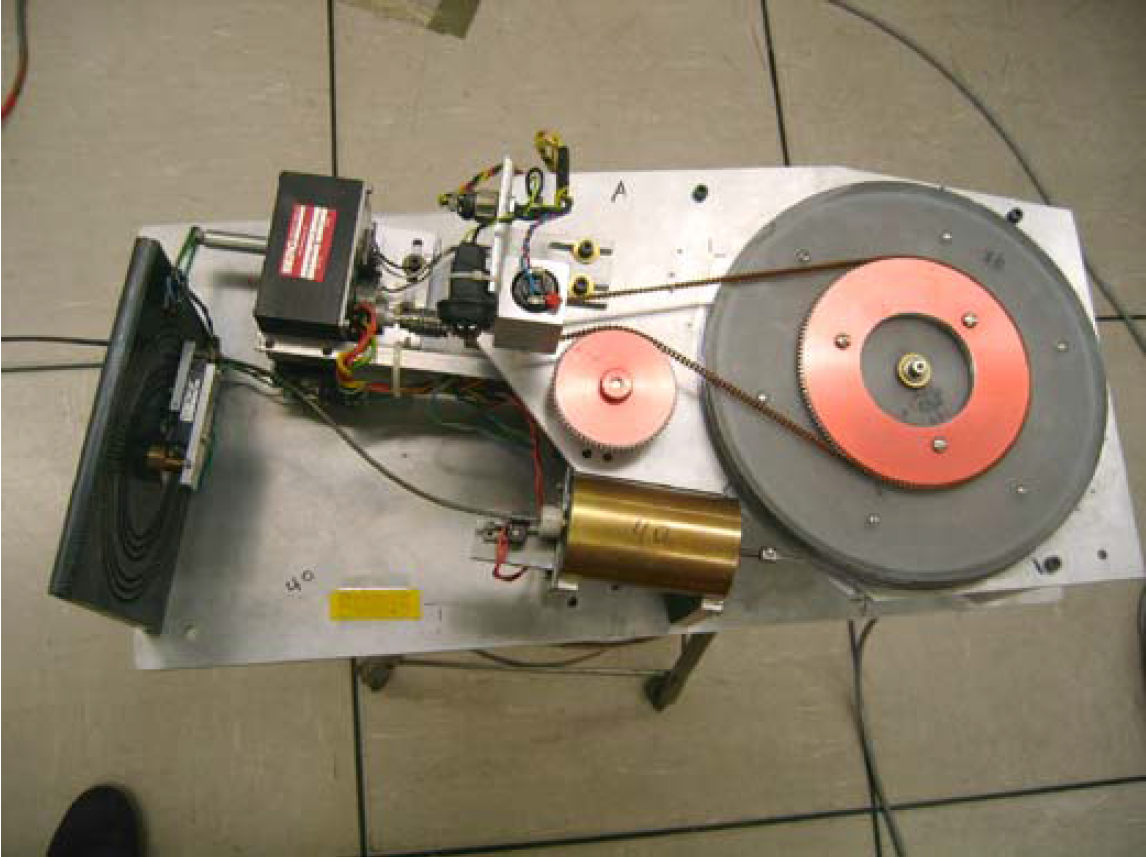
\includegraphics[width=.8\textwidth]{figures/ch_hfcalibration/Source_Driver.png}
      \caption{Source Driver System}
      \label{fig:hf_expsetup_sourcedriver}
   \end{center}
\end{figure}

\subsection{Description of Data Acquisition}
The PMT analog signals are read out by QIEs, standing for charge (Q),
integration (I), and encode (E) \cite{QIE-1}. Each such QIE has 6 differential inputs, which
allow to digitize 6 PMTs simultaneously. Differential inputs are used to subtract
any externally induced noise in signal cables. Each QIE has also 1 fiber-optic
output, which transfers the digitized information to HTRs (HCAL Trigger and
Readout) \cite{HTR}. The output of 8 QIEs is further bundled up into 1 fiber and digitized information is carried to a HTR. Therefore, each HTR receives input from 48 PMTs: 24 PMTs for each tower's HAD channel and 24 PMTs for each tower's EM channel.

A large dynamic range in PMT signal processing is acquired using
a multi-range technique. The input current is simultaneously integrated on all
four ranges, and comparators are used to isolate the lowest range that is not at
full scale. The selected voltage representing the integrated charge is then put
through an on-chip piecewise linear Flash ADC (Analogue to Digital Converter),
with bins weighted according to the time slice (TS) firmware used. For 1 TS, the first 15 bins are weighted by 1, the following 7 bins get a weight 2, the next 4 bins weighted by 3, then 3 bins are weighted by 4, the last 3 bins get a weight 5, providing a range from 0 to 63 ADC counts, with the last
bin (overflow bin) containing all charge above 63 ADC counts. For 2 TS, 10 bins
are weighted 1, 6 bins weighted 2, 5 bins weighted 4, 5 bins weighted 8, 3 bins
weighted 16, 2 bins weighted 32, and 1 bin weighted 62, providing a range from
0 to 194 ADC counts, with the overflow bin containing all charge above 194 ADC
counts. Operations are time multiplexed and pipelined to allow signals to
settle and to make the reset interval the same as the integration interval.
Clocking is provided at the frequency of 40 MHz, with a latency of
100 ns, as the pipeline is four clock cycles deep. Each QIE contains a
set of four capacitors, and only one capacitor is acquiring charge during a
given clock cycle (25 ns). The output is a 5-bit mantissa representing the voltage on
the particular capacitor, and a 2-bit exponent indicating the range
represented by a coded address of the capacitor.

The firmware implemented during radioactive source data acquisition uses a
given TS histogramming mode and operating voltage (OV). In the histogramming
mode, the absorber's response charge is represented across 32 histogram bins,
with the final bin, Bin 32, being the overflow bin containing all data with
charge beyond the particular range. For 1 TS firmware, each TS was recorded in
the histogram. For 2 TS firmware, 2 time slices (25 ns each) are summed and the total was recorded in the histogram. To accommodate
the 2 TS maximum outputs, the expanded QIE bin range described above was used
with respect to 1TS.

Each capacitor from a QIE set fills a separate histogram at the sampling rate,
i.e. latent cycle, and once $6.5535$ $\times$ $10^4$ samples are collected the histogram
is read out by the DAQ (DAQ is a generic acronym used to signify the full chain of data acquisition), two HTR fibers from each HTR half at a time. Data is
saved into event format. Each event containing the histograms read out by all powered HTR
halves - a given PMT's output is stored in every fourth event. This means
that each event represents 6.55 ms of source data. For 1 TS, each sample
was collected over 25 ns, and for 2 TS each sample was collected over
50 ns.